\section{Experiments}
\begin{table*}
    \setlength{\tabcolsep}{12pt}
    \small
    \centering
    \begin{tabular}{llccccccc}
        \toprule
          \multirow{2}{*}{\textbf{PPL}$\downarrow$} & & \multicolumn{3}{c}{\textbf{Llama-2}} & \multicolumn{4}{c}{\textbf{LLaMA}}  \\  \cmidrule(lr){3-5} \cmidrule(lr){6-9}
          & & 7B & 13B & 70B & 7B  & 13B & 30B & 65B\\ \midrule
        FP16 & - & 5.47 & 4.88 & 3.32 & 5.68 &	5.09 & 4.10	& 3.53\\ \midrule
        \multirow{4}{*}{\shortstack{INT3\\g128}} & RTN & 6.66 &	5.52 & 3.98 & 7.01 &	5.88 & 4.88	& 4.24  \\
        & GPTQ &  6.43	& 5.48 & 3.88 & 8.81 & 5.66 & 4.88 & 4.17\\
         & GPTQ-R &  6.42	& 5.41 & 3.86 & 6.53 & 5.64 & 4.74 & 4.21\\
         & \methodshort  & \textbf{6.24} & \textbf{5.32} & \textbf{3.74} & \textbf{6.35} & \textbf{5.52} & \textbf{4.61} & \textbf{3.95} \\ \midrule
         \multirow{4}{*}{\shortstack{INT4\\g128}} & RTN & 5.73 & 4.98 & 3.46& 5.96 & 5.25 & 4.23 & 3.67\\
         & GPTQ &  5.69	& 4.98 & 3.42 & 6.22 & 5.23 & 4.24 & 3.66\\
         & GPTQ-R & 5.63 & 4.99 & 3.43 & 5.83 & 5.20 & 4.22 & 3.66\\
         & \methodshort & \textbf{5.60} & \textbf{4.97} & \textbf{3.41}  & \textbf{5.78} & \textbf{5.19} & \textbf{4.21} & \textbf{3.62}\\
        \bottomrule
    \end{tabular}
    \caption{\methodshort improves over round-to-nearest quantization (RTN) for different model sizes and different bit-precisions. It consistently achieves better perplexity than GPTQ (w/ and w/o reordering) on LLaMA \& Llama-2 models.
    }
    \label{tab:llama_opt_ppl}
\end{table*}

\begin{table}
    \setlength{\tabcolsep}{5pt}
    \small
    \centering
    \begin{tabular}{lcccccccc}
      \toprule
        \textbf{Wikitext2 PPL}$\downarrow$ & Mixtral-8x7B  & Mistral-7B \\  \midrule
      FP16 & 5.94 & 4.14 \\ \midrule
      INT4-g128 & 6.05 & 4.30	 \\
       INT3-g128 & 6.52 & 4.83  \\
      \bottomrule
    \end{tabular}
    \caption{\methodshort quantization results on Mistral-7B-Instruct-v0.2\cite{jiang2023mistral} and Mixtral-8x7B-Instruct-v0.1 model ~\cite{jiang2024mixtral}. The PPL result on wikitext shows that \methodshort can achieve superior quantization performance on different model architectures including LLMs with GQA and Mixture-of-Experts (MoE) models.}
    \label{tab:opt_ppl}
\end{table}



\subsection{Settings}

\myparagraph{Quantization. } We focus on \emph{weight-only grouped} quantization in this work. As shown in previous work~\cite{dettmers2022case, frantar2022gptq}, grouped quantization is always helpful for improving performance/model size trade-off. We used a group size of 128 throughout the work, except otherwise specified. We focus on INT4/INT3 quantization since they are able to mostly preserve the LLMs' performance~\cite{dettmers2022case}. For \methodshort, we used a small calibration set from the Pile~\cite{gao2020pile} dataset in order not to overfit to a specific downstream domain. We used a grid size of 20 to search for the optimal $\alpha$ in Equation~\ref{eq:scale_search_formula}. 

\myparagraph{Models. } We benchmarked our method on LLaMA~\cite{touvron2023llama} and OPT~\cite{opt} families. There are other open LLMs like BLOOM~\cite{scao2022bloom}, but they are generally worse in quality, so we do not include them in our study. We further benchmark an instruction-tuned model Vicuna~\cite{vicuna2023} and visual language models OpenFlamingo-9B~\cite{openflamingo} and LLaVA-13B~\cite{liu2023llava} to demonstrate the generability of our method. 

\myparagraph{Evaluations.} Following previous literature~\cite{dettmers2022llmint8, xiao2022smoothquant, frantar2022gptq, dettmers2022case, zeroquant}, we mainly profiled the quantized models on language modeling tasks (perplexity evaluation on WikiText-2~\cite{merity2016pointer}) since perplexity can stably reflect the LLM's performance~\cite{dettmers2022case}.

\myparagraph{Baselines.} Our primary baseline is vanilla round-to-nearest quantization (RTN). It is actually quite strong when using a small group size like 128~\cite{frantar2022gptq, dettmers2022case}. We also compare with a state-of-the-art method GPTQ~\cite{frantar2022gptq} for LLM weight quantization. For GPTQ, we also compare with an updated version that uses a ``reorder'' trick (denoted as GPTQ-Reorder or GPTQ-R). Other techniques like ZeroQuant~\cite{zeroquant}, AdaRound~\cite{nagel2020up}, and BRECQ~\cite{li2021brecq} rely on backpropagation to update the quantized weights, which may not easily scale up to large model sizes; they also do not outperform GPTQ~\cite{frantar2022gptq}, thus not included for study. 


\subsection{Evaluation}
\definecolor{winblue}{RGB}{114, 147, 182}

\begin{figure}%
    \centering
     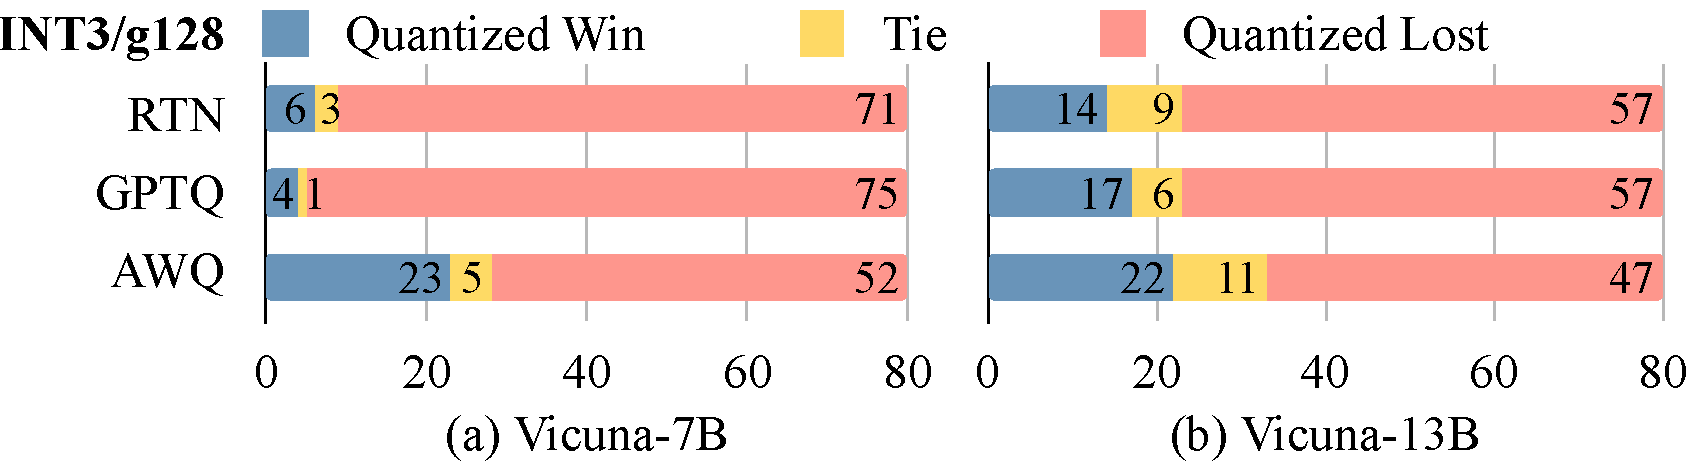
\includegraphics[width=0.5\textwidth]{figures/vicuna_gpt4_eval_small.pdf}
    \caption{Comparing INT3-g128 quantized Vicuna models with FP16 counterparts under GPT-4 evaluation protocol~\cite{vicuna2023}. More winning cases (in 
    \textcolor{winblue}{blue}) indicate better performance. \methodshort consistently improves the quantized performance compared to RTN and GPTQ~\cite{frantar2022gptq}, showing generalization to instruction-tuned models.
    } 
    \label{fig:vicuna_gpt4_eval}
\end{figure}

    



\begin{table*}%
    \small
    \setlength{\tabcolsep}{11pt}
    
    \centering
    \begin{tabular}{llcccccc}
        \toprule
        \multicolumn{2}{l}{\textbf{COCO (CIDEr $\uparrow$)}} & 0-shot & 4-shot & 8-shot & 16-shot & 32-shot & \emph{$\Delta$(32-shot)} \\  \midrule
    FP16 & - & 63.73 & 72.18 & 76.95 & 79.74 & 81.70  & - \\ \midrule
    \multirow{3}{*}{\shortstack{INT4\\g128}} & RTN & 60.24 & 68.07 & 72.46 & 74.09 & 77.13 & -4.57 \\ 
    & GPTQ & 59.72 & 67.68 & 72.53 & 74.98 & 74.98 & -6.72 \\ %
    & \methodshort & \textbf{62.57} & \textbf{71.02} & \textbf{74.75} & \textbf{78.23} & \textbf{80.53} & \textbf{-1.17} \\ \midrule
     \multirow{3}{*}{\shortstack{INT3\\g128}} & RTN & 46.07 & 55.13 & 60.46 & 63.21 & 64.79 & -16.91\\ 
    & GPTQ & 29.84 & 50.77 & 56.55 & 60.54 & 64.77 & -16.93\\ %
    & \methodshort & \textbf{56.33} & \textbf{64.73} & \textbf{68.79} & \textbf{72.86} & \textbf{74.47} & \textbf{-7.23}\\
        \bottomrule
    \end{tabular}
    \caption {Quantization results of a visual language model OpenFlamingo-9B~\cite{openflamingo} on COCO Captioning datasets. \method{} outperforms existing methods under zero-shot and various few-shot settings, demonstrating the generability to different modalities and in-context learning workloads. \method{} reduces the quantization degradation (32-shot) from 4.57 to 1.17 under INT4-g128, providing 4$\times$ model size reduction with negligible performance loss. 
    }
    \label{tab:openflamingo}
\end{table*}

\begin{table*}
    \setlength{\tabcolsep}{5pt}
    \small
    \centering
\begin{tabular}{@{}lccccccccccc@{}}
\toprule
\textbf{Model (Accuracy$\uparrow$)} & VQAv2 & GQA & VizWiz & SQA-I & VQA-T & POPE & MME & MMB & SEED & llava-bench & MM-Vet \\
\midrule
VILA-7B           & 80.3 & 63.1 & 59.6   & 68.0  & 62.6  & 86.3  & 1489.4 & 69.8	   & 61.7 & 75.2        & 35.1   \\
VILA-7B-AWQ       & 80.1 & 63.0 & 57.8   & 68.0  & 61.9  & 85.3  & 1486.3 & 68.8   & 61.3 & 75.8        & 35.9   \\
VILA-13B          & 80.5 & 63.6 & 63.1   & 70.5  & 64.0  & 86.3  & 1553.6 & 73.8   & 62.8 & 78.3        & 42.6   \\
VILA-13B-AWQ      & 80.4 & 63.6 & 63.0   & 71.2  & 63.5  & 87.0  & 1552.9 & 73.6   & 62.2 & 77.6        & 42.0   \\
\bottomrule
\end{tabular}
\caption{INT4-g128 results of VILA-7B and VILA-13B~\cite{lin2023vila} on 11 visual-language benchmarks. \methodshort consistently shows lossless performance on all benchmarks. Benchmark names are abbreviated due to space limits. VQA-v2~\cite{goyal2017vqav2}; GQA~\cite{hudson2019gqa}; VisWiz~\cite{gurari2018vizwiz}; SQA$^\text{I}$: ScienceQA-IMG~\cite{lu2022learn}; VQA$^\text{T}$: TextVQA~\cite{singh2019textvqa}; POPE~\cite{li2023pope}; MME~\cite{fu2023mme}; MMB: MMBench~\cite{liu2023mmbench}; MMB$^\text{CN}$: MMBench-Chinese~\cite{liu2023mmbench}; SEED: SEED-Bench~\cite{li2023seed}; LLaVA$^\text{W}$: LLaVA-Bench (In-the-Wild)~\cite{liu2023llava}; MM-Vet~\cite{yu2023mmvet}.}
\label{tab:vila_acc}

\end{table*}



\myparagraph{Results on LLaMA models.}
We focus on LLaMA models (LLaMA~\cite{touvron2023llama} and Llama-2~\cite{touvron2023llama2}) due to their superior performance compared to other open-source LLMs~\cite{opt, scao2022bloom}; it is also the foundation of many popular open-source models~\cite{alpaca, vicuna2023}. We evaluate the perplexity before and after quantization in Table~\ref{tab:llama_opt_ppl}. 
\methodshort consistently outperforms round-to-nearest (RTN) and GPTQ~\cite{frantar2022gptq} (w/ and w/o reordering) across different model scales (7B-70B) and generations. 

\myparagraph{Results on Mistral / Mixtral models.}
We also evaluated \methodshort on the Mistral and Mixtral models, which are among the most popular open-source LLMs and Mixture-of-Experts (MoE) models, respectively~\cite{jiang2023mistral, jiang2024mixtral}. The results indicate that \methodshort achieves superior performance on both the Mistral and Mixtral models. This demonstrates that \methodshort is effective across various model architectures.






\begin{figure*}[t]
    \centering
     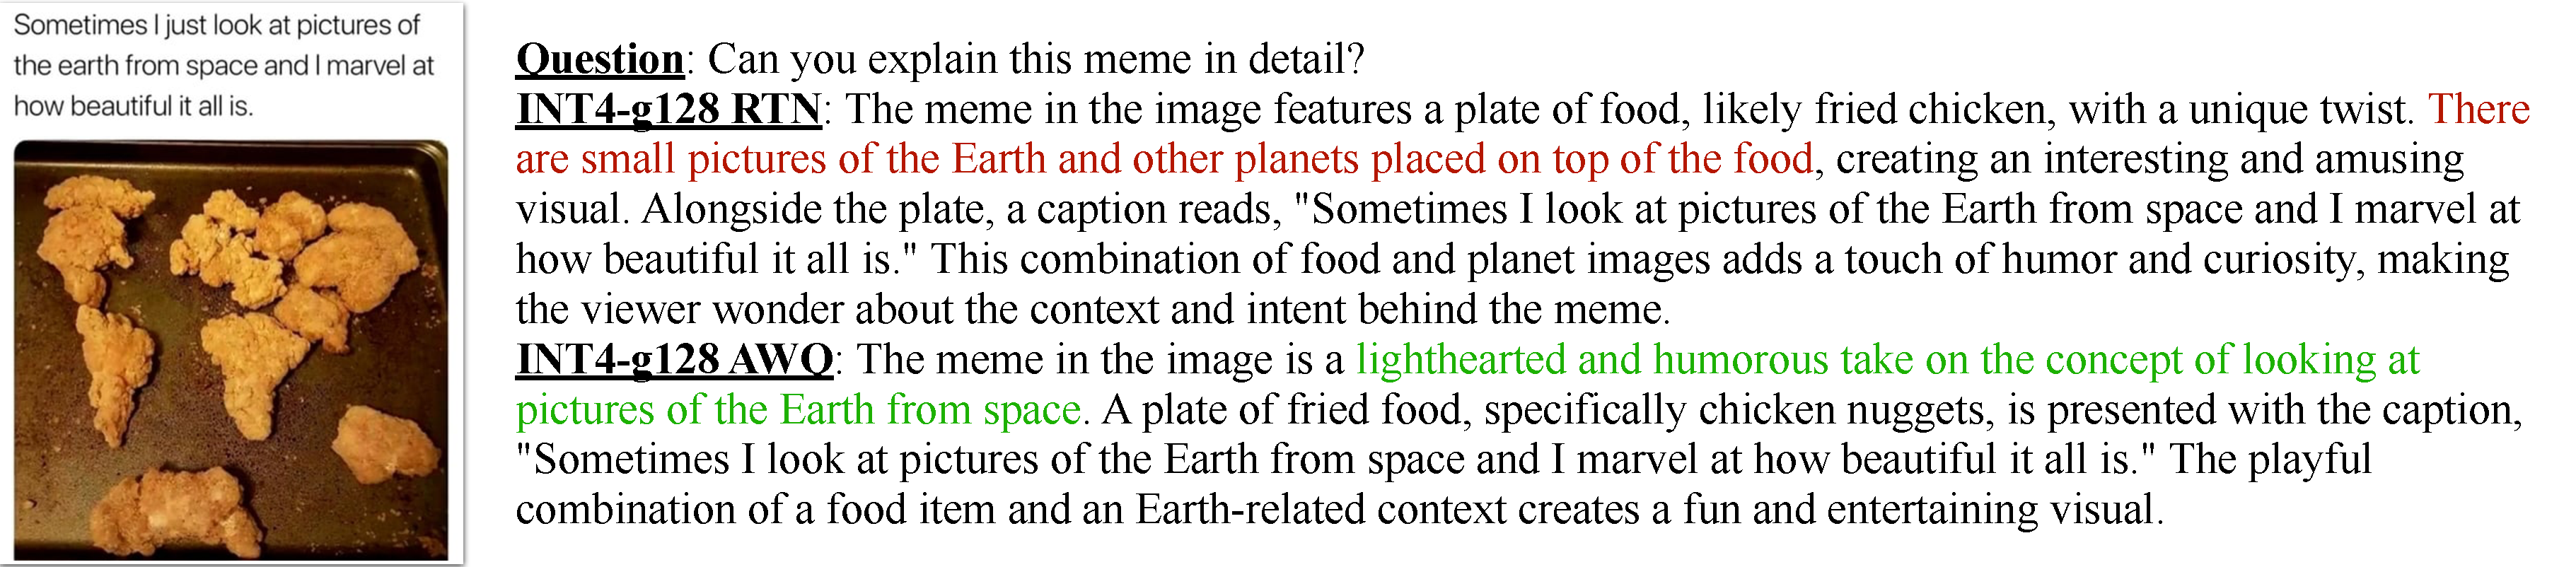
\includegraphics[width=\textwidth]{figures/visual_reasoning.pdf}
    \caption{Visual reasoning examples from LLaVA-13B model~\cite{liu2023llava}. \methodshort improves over the round-to-nearest (RTN) baseline, providing more reasonable answers. We color the text to show the \textcolor{codegreen}{correct} or \textcolor{red}{wrong} responses. 
    } 
    \label{fig:visual_reasoning}
\end{figure*}


\begin{figure*}[t]
    \centering
     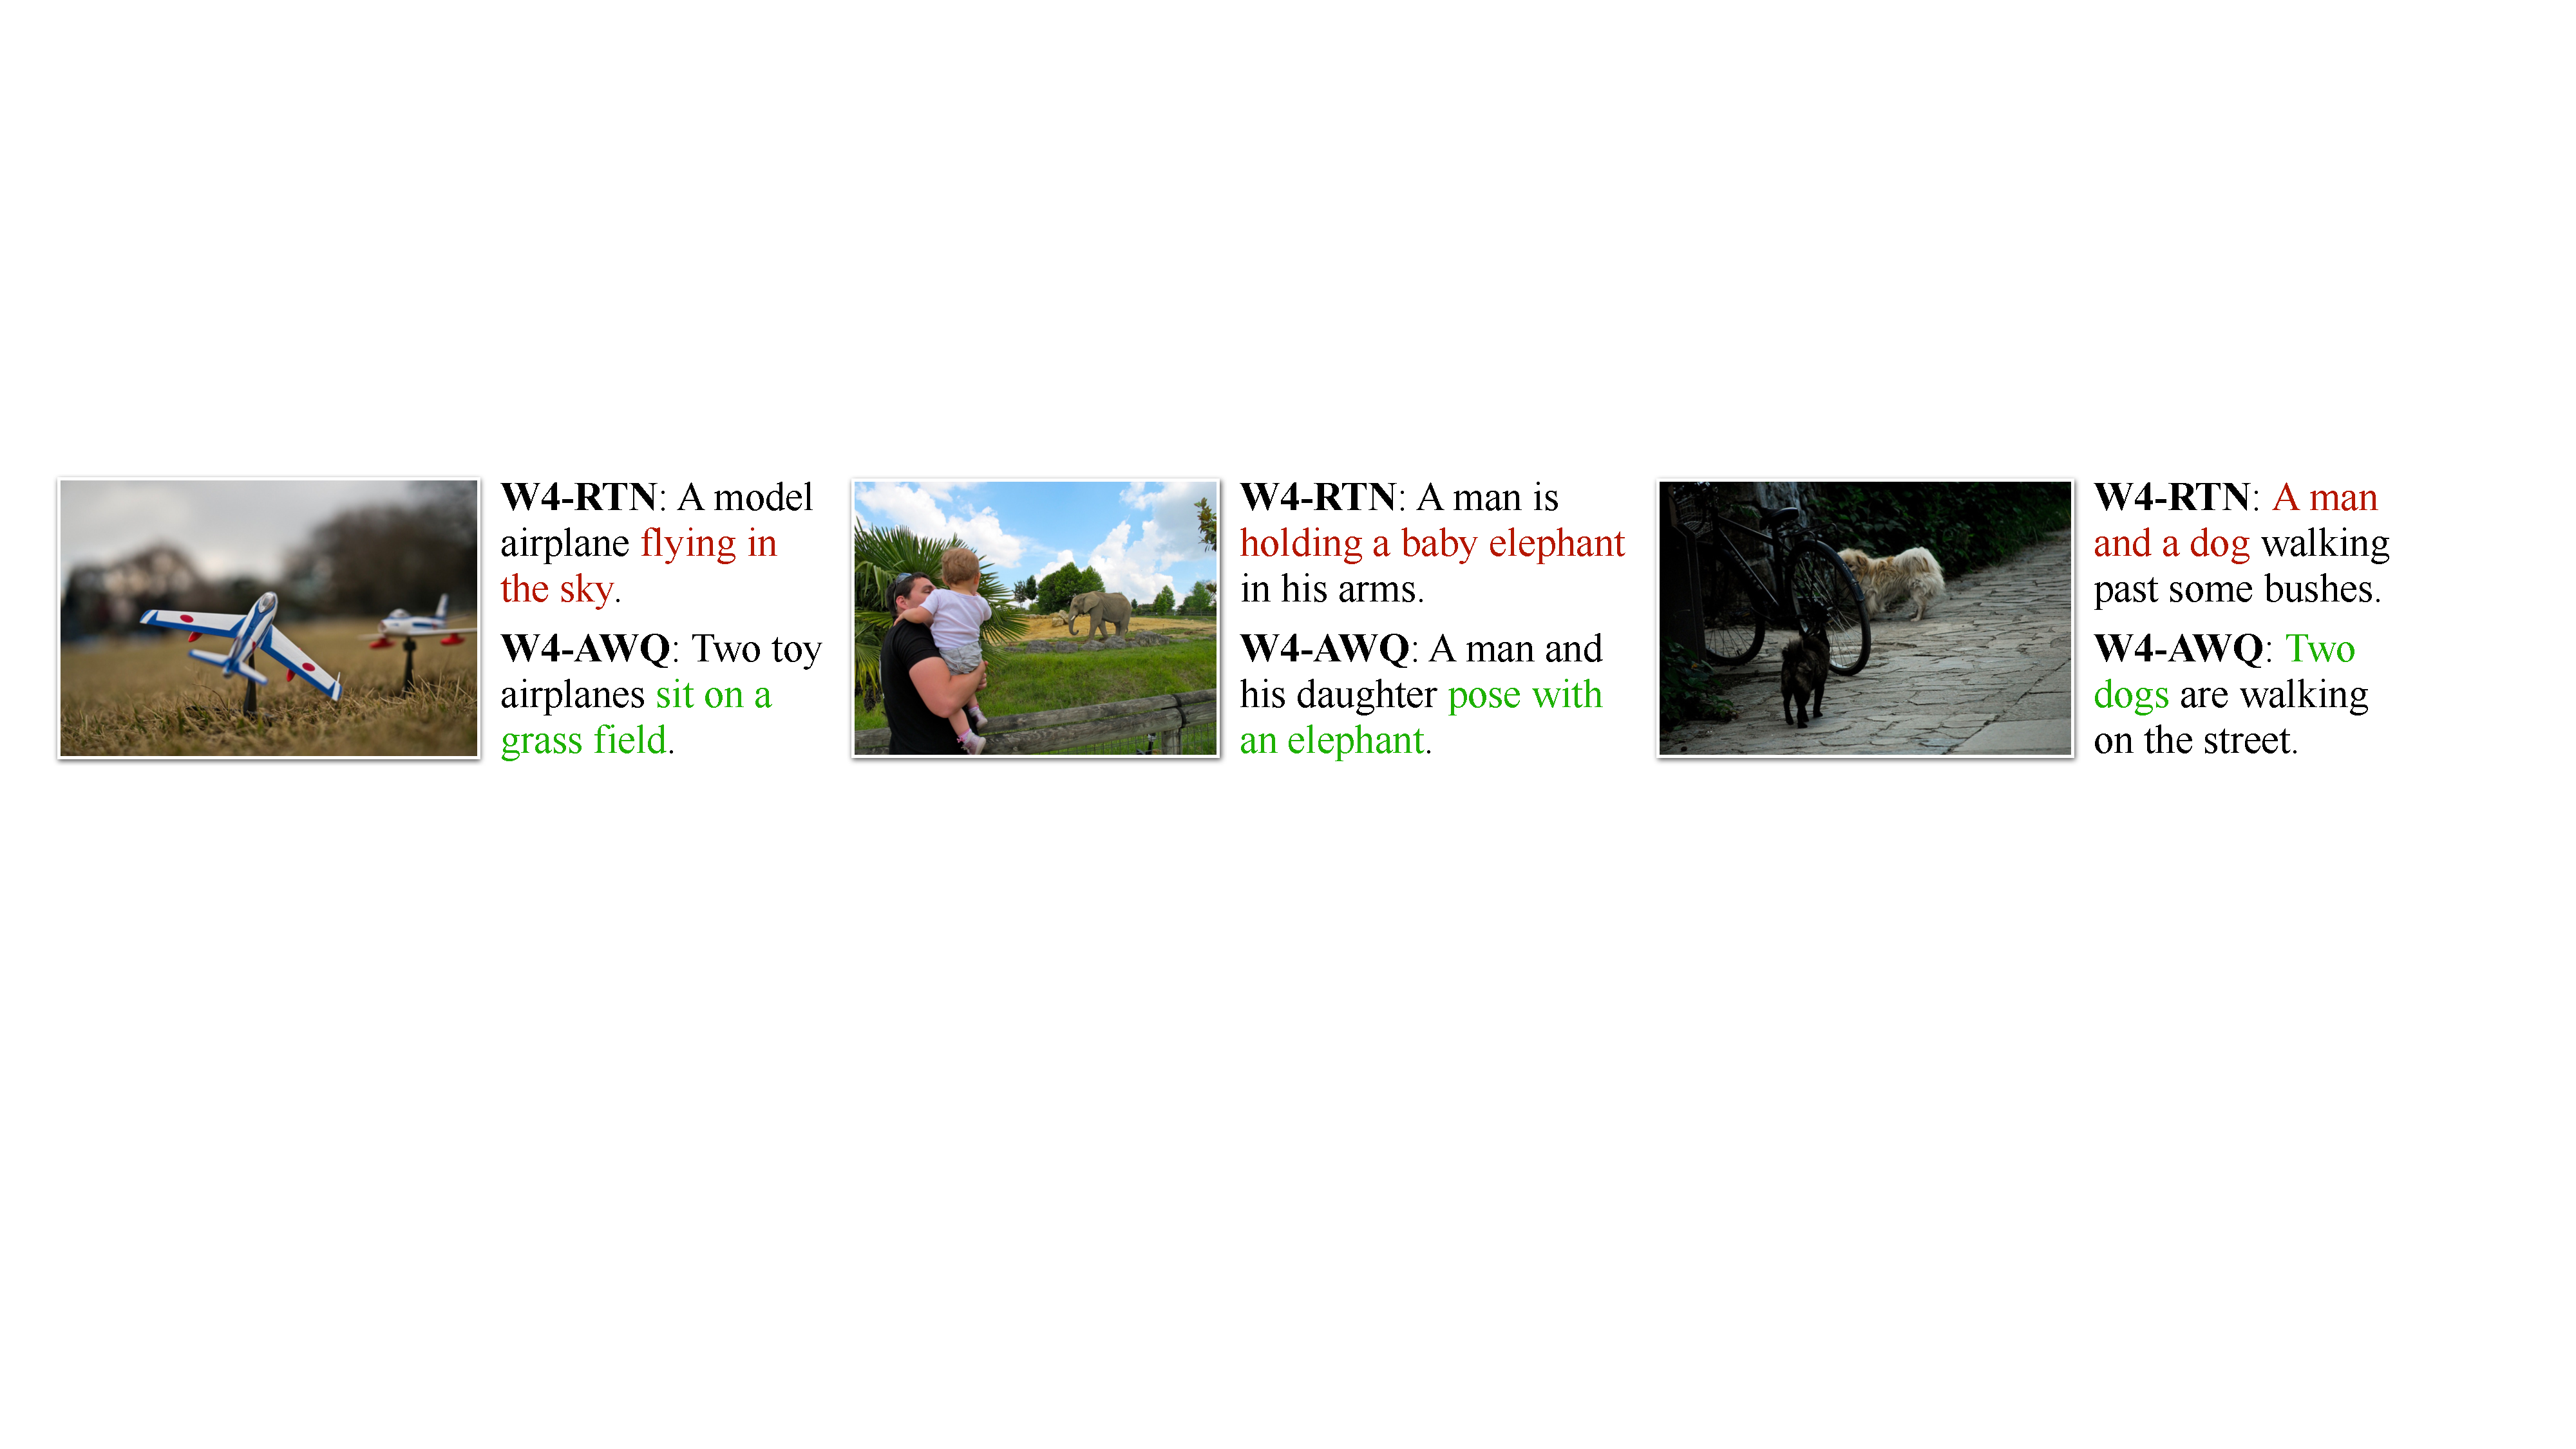
\includegraphics[width=\textwidth]{figures/coco_caption_samples_w4.pdf}
    \caption{Qualitative results of quantized OpenFlamingo-9B~\cite{openflamingo} on COCO captioning dataset (4-shot, INT4-g128 quantization). Our method significantly improves the captioning quality compared to the round-to-nearest (RTN) baseline. We color the text to show the \textcolor{codegreen}{correct} or \textcolor{red}{wrong} captions. }
    \label{fig:coco_sample}
\end{figure*}



\myparagraph{Quantization of instruction-tuned models.}
Instruction tuning can significantly improve the models' performance and usability 
~\cite{wei2021finetuned,sanh2021multitask,ouyang2022training,chung2022scaling}. It has become an essential procedure before model deployment. We further benchmark our method's performance on a popular instruction-tuned model Vicuna~\cite{vicuna2023} in Figure~\ref{fig:vicuna_gpt4_eval}. We used the GPT-4 score to evaluate the quantized models' performance against the FP16 counterpart on 80 sample questions~\cite{vicuna2023}.
We compare the responses with both orders (quantized-FP16, FP16-quantized) to get rid of the ordering effect (we found GPT-4 tends to increase the rating of the first input), leading to 160 trials. 
\methodshort consistently improves the INT3-g128 quantized Vicuna models over RTN and GPTQ under both scales (7B and 13B), demonstrating the generability to instruction-tuned models.  
    



\begin{table}
    \small
    \setlength{\tabcolsep}{2pt}
    
    \centering
    \begin{tabular}{llcccccc}
        \toprule
        \textbf{MBPP (7B)} & pass@1 & pass@10 \\  \midrule
    FP16 & 38.53 & 49.77 \\ \midrule
    RTN & 37.51 & 48.49  \\ 
    GPTQ & 31.97 & 44.75  \\ %
    \methodshort & \textbf{40.64} & \textbf{49.25}  \\ 
        \bottomrule
    \end{tabular}
    \begin{tabular}{llcccccc}
        \toprule
        \textbf{GSM8K} & 7B & 13B & 70B \\  \midrule
    FP16  & 13.87 & 26.16 & 56.41 \\ \midrule
    RTN & 11.07 & 21.23 & 53.98 \\ 
    GPTQ & 12.13 & 24.26 & 56.03  \\ %
    \methodshort & \textbf{13.57} & \textbf{25.25} & \textbf{56.40} \\ 
        \bottomrule
    \end{tabular}
    \caption {INT4-g128 quantization results of CodeLlama-7b-Instruct-hf on MBPP dataset and Llama-2 (7B/13B/70B) on GSM8K dataset. AWQ outperforms existing methods on programming and math datasets, demonstrating the generability to different scenarios and evaluation settings. Notably, AWQ under the INT4-g128 configuration demonstrates comparable performance to the original FP16 model across both datasets.}
    \label{tab:code_and_math}
\end{table}



\myparagraph{Quantization of multi-modal language models.} Large multi-modal models (LMMs) or visual language models (VLMs) are LLMs augmented with vision inputs~\cite{alayrac2022flamingo,li2023blip,koh2023grounding,driess2023palm,zhang2023llama,liu2023llava}. Such models are able to perform text generation conditioned on image/video inputs. Since our method does not have the overfitting issue to the calibration set, it can be directly applied to VLMs to provide accurate and efficient quantization. 
We perform experiments with the OpenFlamingo-9B model~\cite{openflamingo} (an open-source reproduction of~\cite{alayrac2022flamingo}) on COCO captioning~\cite{chen2015microsoft} dataset (Table~\ref{tab:openflamingo}). We measured the average performance of 5k samples under different few-shot settings. We only quantize the language part of the model since it dominates the model size. 
\methodshort outperforms existing methods under zero-shot and various few-shot settings, demonstrating the generability to different modalities and in-context learning workloads. It reduces the quantization degradation (32-shot) from 4.57 to 1.17 under INT4-g128, providing 4$\times$ model size reduction with negligible performance loss. 
To further demonstrate the generability of \methodshort, we also evaluated \methodshort on one of the SoTA multi-image visual language models: VILA. The result in Table~\ref{tab:vila_acc} shows that \methodshort achieves lossless quantization performance on 11 visual-language benchmarks.
We further provide some qualitative captioning results in Figure~\ref{fig:coco_sample} to show our advantage over RTN.  
Our method provides a push-the-button solution for LMM/VLM quantization. It is the \emph{first} study of VLM low-bit quantization to the best of our knowledge.

\begin{figure*}
    \centering
     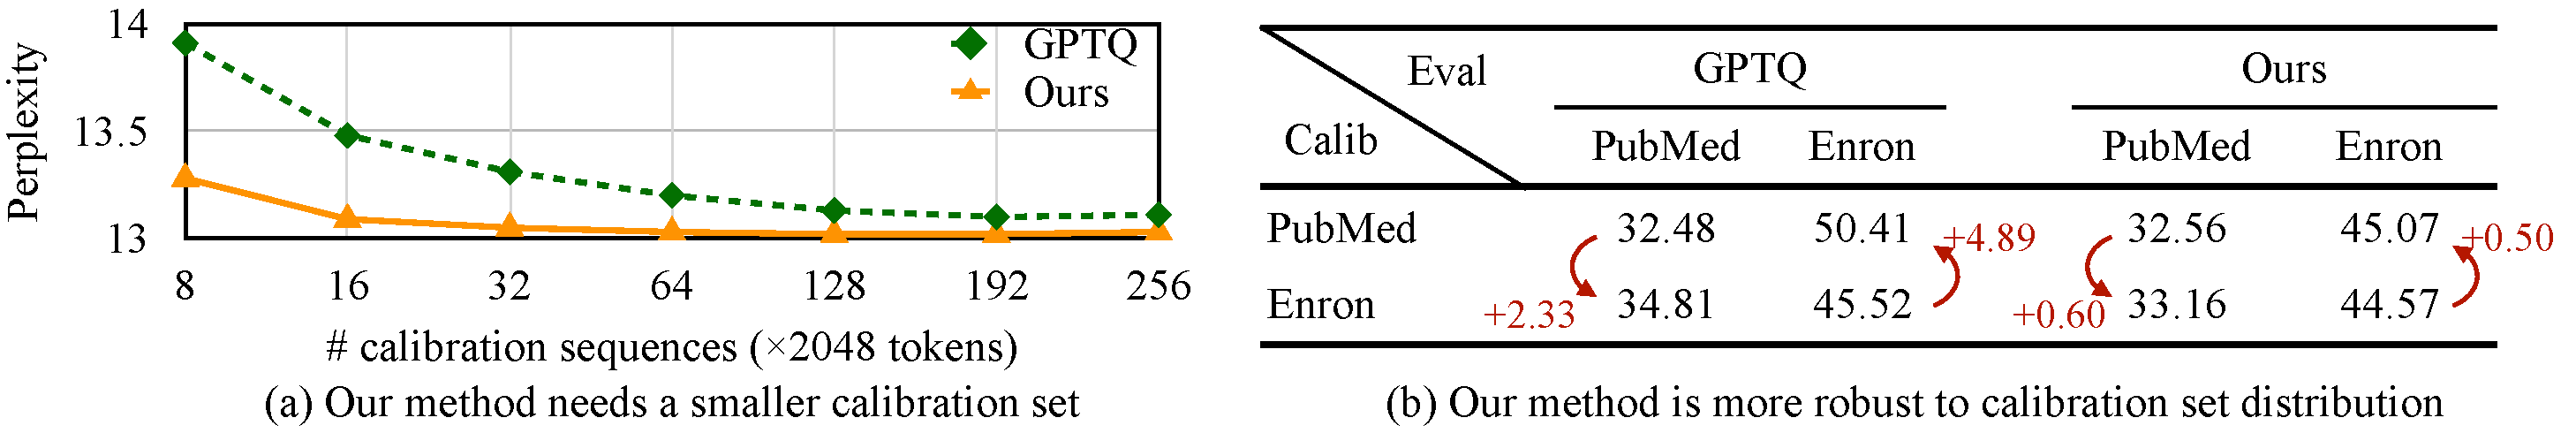
\includegraphics[width=\textwidth]{figures/calib_set_ablation_small.pdf}
    \caption{\textbf{Left:} \methodshort needs a much smaller calibration set to reach a good quantized performance. It can achieve better perplexity using 10$\times$ smaller calibration set compared to GPTQ. \textbf{Right:} Our method is more robust to the calibration set distribution. Overall, using the same calibration and evaluation distribution works the best (PubMed-PubMed, Enron-Enron). But when using a different calibration distribution (PubMed-Enron, Enron-PubMed), \methodshort only increases the perplexity by 0.5-0.6, while GPTQ has 2.3-4.9 worse perplexity. All experiments are done with the OPT-6.7B model under INT3-g128 quantization.}
    \label{fig:calib_set_ablation}
\end{figure*}


\begin{figure*}[t]
    \centering
     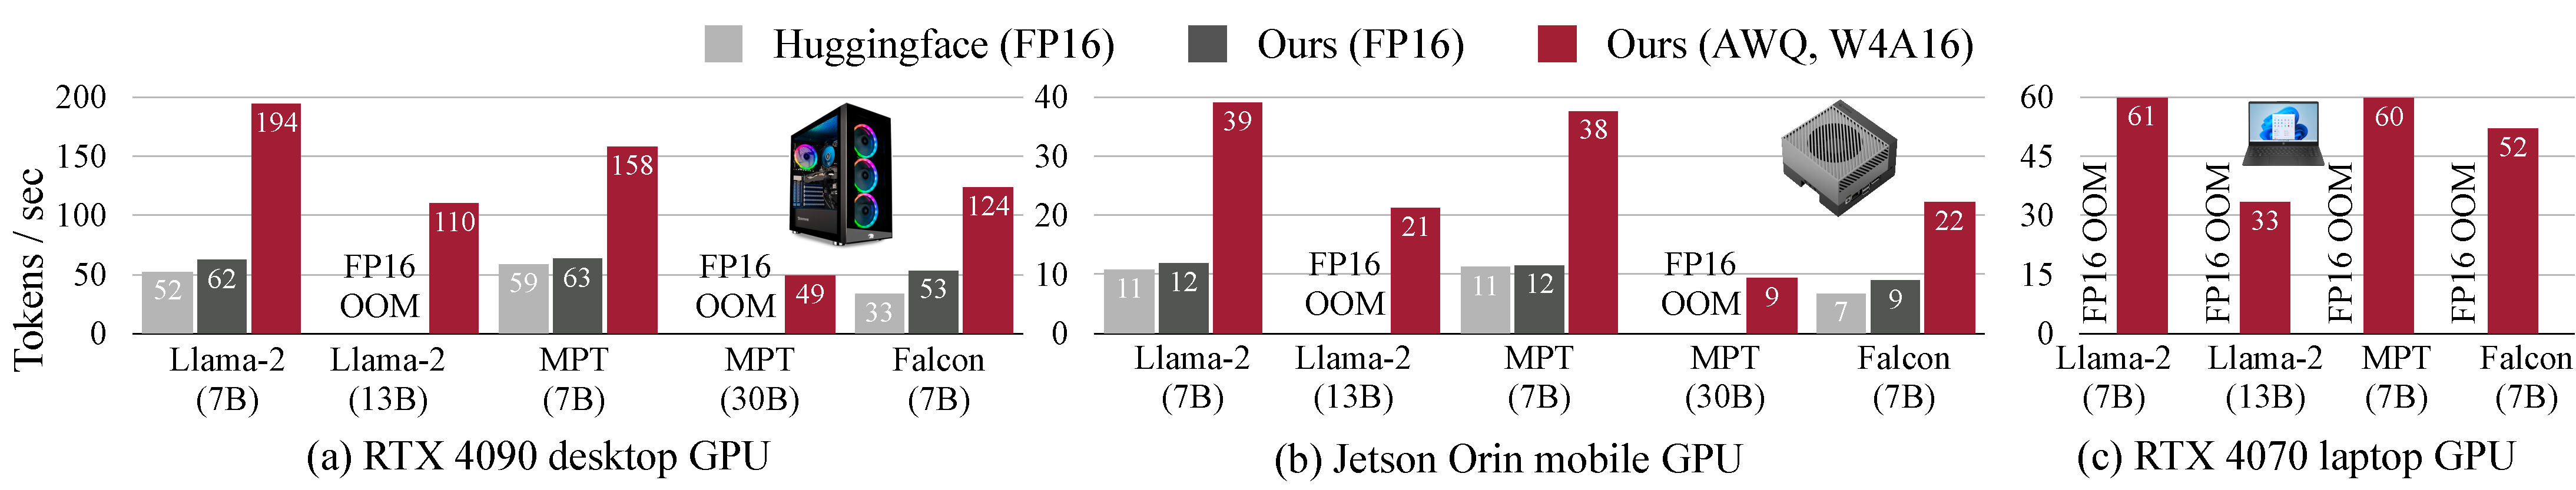
\includegraphics[width=\textwidth]{figures/speedup.pdf}
\caption{\system provides a turn-key solution to transform the theoretical memory footprint reduction into a quantifiable speedup. As a result, \system is up to \textbf{3.9$\times$} and \textbf{3.5$\times$} faster than the FP16 implementation from Huggingface on 4090 (desktop GPU) and Orin (mobile GPU), respectively. AWQ also democratizes Llama-2-13B deployment on laptop GPUs (4070) with merely 8GB memory.} %
    \label{fig:kernel_speedup}
\end{figure*}


\begin{figure*}[t]
    \centering
     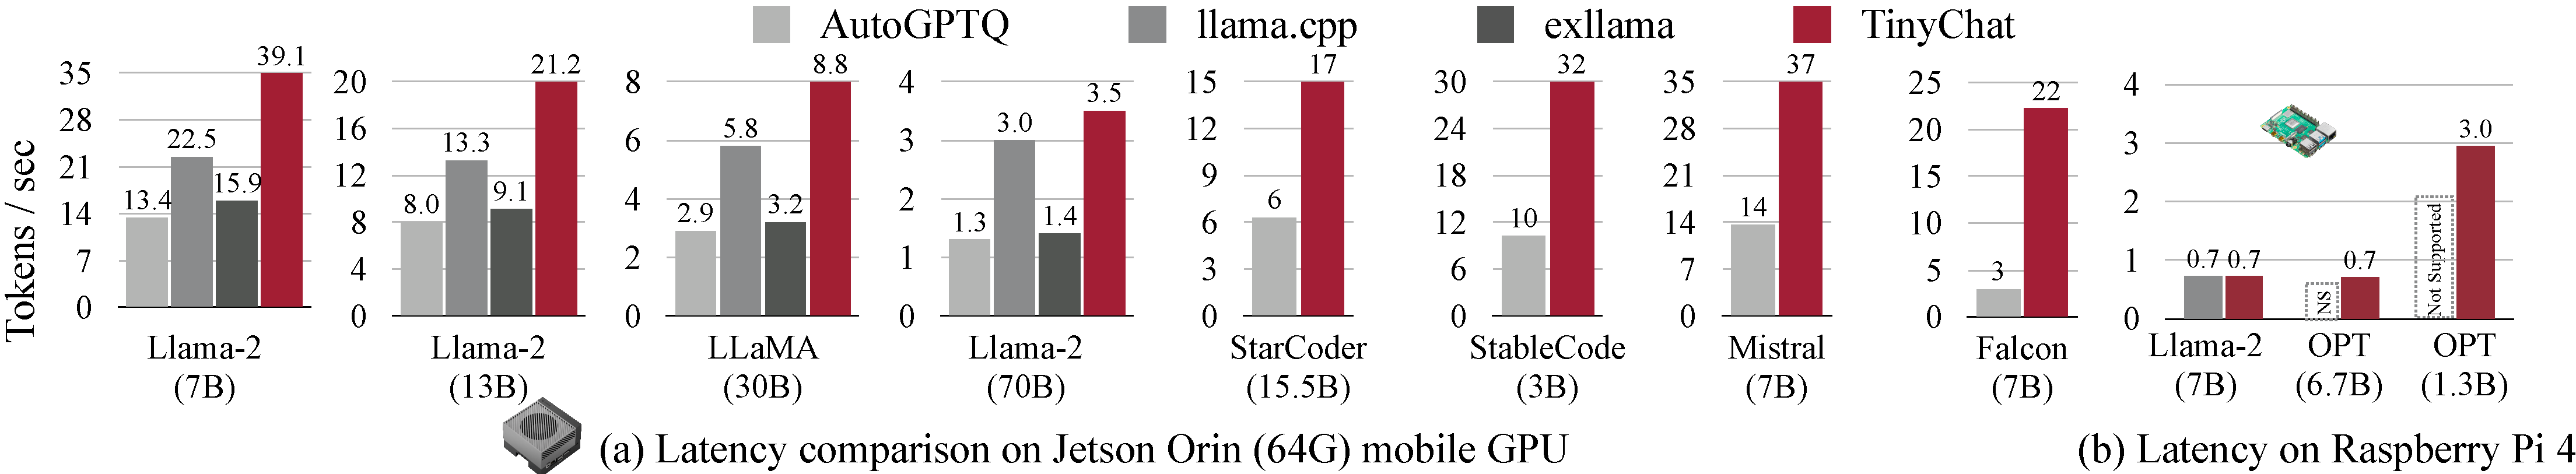
\includegraphics[width=\textwidth]{figures/speedup_comparisons.pdf}
\caption{\system offers \textbf{1.2-3.0$\times$} speedup over existing systems when running 4-bit quantized Llama models on NVIDIA Jetson Orin. It also supports a diverse range of general-purpose and coding-specific LLMs with at least \textbf{2.6$\times$} speedup over AutoGPTQ, which also supports all these workloads. Moreover, \system seamlessly operates on Raspberry Pi and enables the deployment of LLMs with up to 7 billion parameters on extremely resource-constrained IoT devices.} %
    \label{fig:kernel_speedup_comparisons}
\end{figure*}

\begin{table}
\small
    \setlength{\tabcolsep}{3pt}
    
    \centering
    \begin{tabular}{llccccc}
        \toprule
          \textbf{OPT (Wiki PPL$\downarrow$)} & 1.3B & 2.7B & 6.7B & 13B & 30B  \\  \midrule
        FP16& 14.62 & 12.47 & 10.86 & 10.13 & 9.56 \\ \midrule
        RTN & 10476 & 193210 & 7622 & 17564 & 8170 \\
        GPTQ & 46.67 & 28.15 & 16.65 & 16.74 &  11.75 \\ \cmidrule(lr){2-6}
        \methodshort+GPTQ & \textbf{35.71} & \textbf{25.70} & \textbf{15.71} & \textbf{13.25} & \textbf{11.38}   \\
        \bottomrule
    \end{tabular}
    \caption{Our method is orthogonal to GPTQ: it further closes the performance gap under extreme low-bit quantization (INT2-g64) when combined with GPTQ. Results are WikiText-2 perplexity of OPT models.  }
    \label{tab:int2}
\end{table}


\myparagraph{Visual reasoning results.}
We further provide some qualitative visual reasoning examples of the LLaVA-13B~\cite{liu2023llava} model in Figure~\ref{fig:visual_reasoning}. \methodshort improves the responses compared to round-to-nearest (RTN) for INT4-g128 quantization, leading to more reasonable answers. In this first example, the \methodshort model can understand the meme as it resembles the Earth when looking from space, while RTN produces wrong descriptions (marked in \textcolor{red}{red}). %

\myparagraph{Results on programming and math tasks}
To further evaluate the performance of AWQ on tasks involving complex generations, we also tested AWQ on MBPP~\cite{austin2021program} and GSM8K~\cite{cobbe2021training}. MBPP~\cite{austin2021program} consists of around 1,000 Python programming problems, designed to be solvable by entry level programmers, covering programming fundamentals, standard library functionality, etc. GSM8K~\cite{cobbe2021training} was created to support the task of question answering on basic mathematical problems that require multi-step reasoning. We quantize CodeLlama-7b-Instruct-hf and Llama-2 to INT4-g128 and perform experiments on programming and math datasets (Table~\ref{tab:code_and_math}). AWQ outperforms existing methods on both datasets, demonstrating the generability to complex generation. AWQ under the INT4-g128 configuration demonstrates comparable
performance to the original FP16 model on both datasets.


\myparagraph{Extreme low-bit quantization.}
We further quantize LLM to INT2 to accommodate limited device memory (Table~\ref{tab:int2}). RTN completely fails, and \methodshort brings significant perplexity improvement on top of GPTQ.%
Our method is orthogonal to GPTQ.
We can combine our method with GPTQ to further improve the INT2 quantization performance, making it a more practical setting. 

\subsection{Data Efficiency and Generalization}
\label{sec:ablation_study}
\myparagraph{Better data-efficiency for the calibration set.} Our method requires a smaller calibration set since we do not rely on regression/backpropagation; we only measure the average activation scale from the calibration set, which is data-efficient.
To demonstrate the idea, we compare the perplexity of the OPT-6.7B model with INT3-g128 quantization in Figure~\ref{fig:calib_set_ablation} (a). \methodshort needs a much smaller calibration to reach a good quantized performance; it can achieve better perplexity using 10$\times$ smaller calibration set compared to GPTQ (16 sequences \emph{v.s.} 192 sequences).

\myparagraph{Robust to the calibration set distributions. }
Our method is less sensitive to the calibration set distribution since we only measure the average activation scale from the calibration set, which is more generalizable across different dataset distributions. We further benchmarked the effect of the different calibration set distributions in Figure~\ref{fig:calib_set_ablation}(b). We took two subsets from the Pile dataset~\cite{gao2020pile}: PubMed Abstracts and Enron Emails~\cite{klimt2004enron}. We use each of the subsets as the calibration set and evaluate the quantized model on both sets (the calibration and evaluation sets are split with no overlapping; we used 1k samples for evaluation). Overall, using the same calibration and evaluation distribution works the best (PubMed-PubMed, Enron-Enron). But when using a different calibration distribution (PubMed-Enron, Enron-PubMed), \methodshort only increases the perplexity by 0.5-0.6, while GPTQ has 2.3-4.9 worse perplexity. This demonstrates the robustness of \methodshort to the calibration set distribution. 

\subsection{Speedup Evaluation}
\begin{table}
    \setlength{\tabcolsep}{5pt}
    \small
    \centering
    \begin{tabular}{lcccc} \toprule
\textbf{Model (Throughput$\uparrow$)}          & Precision & A100 & 4090 & Orin \\ \midrule
VILA-7B      & FP16      & 81.6              & 58.5              & 11.5              \\
VILA-7B-AWQ  & W4A16     & 155.3             & 168.1             & 35.6              \\ \midrule
VILA-13B     & FP16      & 48.5              & OOM               & 6.1               \\
VILA-13B-AWQ & W4A16     & 102.1             & 99.0              & 17.5 \\\bottomrule             
\end{tabular}
    \caption{\system also enables seamless deployment of VILA~\cite{lin2023vila}, a state-of-the-art visual-language model, on multiple GPU platforms. Leveraging our 4-bit AWQ quantization, \system accelerates VILA-7B by up to \textbf{3.1$\times$} and VILA-13B by up to \textbf{2.9$\times$}.}
    \label{tab:vila_latency}
\end{table}





\myparagraph{Settings.} In Figure~\ref{fig:kernel_speedup}, we demonstrate the system acceleration results from \system. \system optimizes both linear layers and layers that do not have quantized weights. We conduct benchmarking experiments on RTX 4090 and Jetson Orin following the protocol described in exllama~\footnote{\url{https://github.com/turboderp/exllama}}. We perform batch size = 1 inference for all LLMs using a fixed prompt length of 4 tokens. We generate 200 tokens for each inference run and calculate the median latency as the final result.

\myparagraph{Results.} As in Figure~\ref{fig:kernel_speedup}(a), \system brings \textbf{2.7-3.9$\times$} speedup to three families of LLMs (Llama-2, MPT and Falcon) on 4090 compared with the Huggingface FP16 implementation. For Llama-2-7B, we improve the inference speed from 52 tokens/s to 62 tokens/s through FP16 kernel fusion. On top of the stronger FP16 baseline, we further harvest \textbf{3.1$\times$} additional speedup from the fast quantized linear kernels. For Falcon-7B, the official implementation did not support KV cache correctly during the inference time, and thus it is significantly slower than other models. In this case, our FP16 optimizations bring about a larger speedup of \textbf{1.6$\times$}. On the laptop 4070 GPU with only 8GB memory, we are still able to run Llama-2-13B models at 33 tokens/s, while the FP16 implementation cannot fit 7B models. We also demonstrate visual-language model~\cite{lin2023vila} acceleration results in Table \ref{tab:vila_latency}. \system brings about \textbf{3$\times$} speedup to both VILA-7B and VILA-13B on NVIDIA Jetson Orin. Notably, we implement the forward pass for all AWQ models using native PyTorch APIs, and this code is reused across various GPU architectures. Hence, \system offers exceptional extensibility. %


\myparagraph{Comparisons against other systems.}
We compare \system against existing edge LLM inference systems AutoGPTQ, llama.cpp and exllama in Figure~\ref{fig:kernel_speedup_comparisons}. Our system achieves up to 1.7$\times$ speedup over llama.cpp on Orin. Furthermore, llama.cpp and exllama exhibit limited adaptability, primarily tailored for LLaMA and Llama-2 models. In contrast, our \system supports a wide range of applications, including StarCoder~\cite{li2023starcoder}, StableCode (GPT-NeoX)~\cite{black2022gpt}, Mistral~\cite{jiang2023mistral}, and Falcon~\cite{penedo2023refinedweb} while consistently delivering significant speedup over AutoGPTQ. \system even democratizes LLM deployment on extremely resource-constrained Raspberry Pi 4B, achieving 0.7 tokens/s for 7B models. 















